\section*{PyAjedrez}

El ajedrez es uno de los juegos de tablero mas conocidos del mundo. En este intensivo haremos una versión reducida del juego. Siguiendo una versión simplificada de sus reglas.

En este intensivo trabajaremos con un tablero mas chico, con menos piezas y sin considerar la mecánica de
los jaques, si no que veremos la lógica para aprobar o descartar ciertas ideas de movimiento de piezas, cálculos
de puntajes, y manejo de instrucciones. Consideraremos además el sistema de coordenadas que muestra la
gura 1.

\vspace{3cm}

\begin{center}
    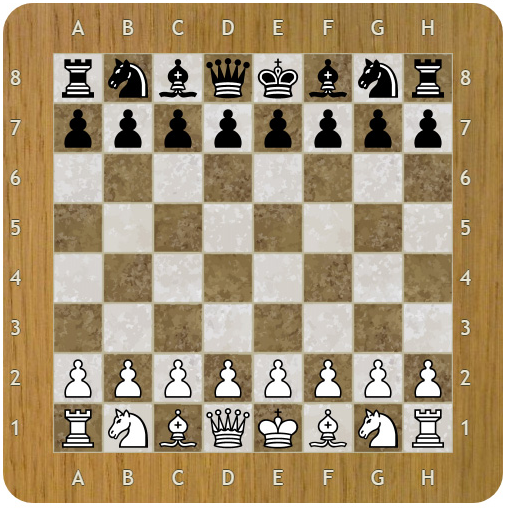
\includegraphics[scale=1]{Imagenes/tablero.png}
\end{center}

